\chapter{Properties of Trigonometric Functions}
I had originally written the section on the properties of trigonometric functions as part of the "Basic Trigonometric Functions" chapter, but it got \textit{really} long. Long enough that I eventually decided to make it it's own chapter.

I'll begin with the period and then continue to frequency.
\section{Period For The Sine and Cosine Functions}
The period of a function is how long it takes to complete one full cycle, where one full cycle is how long it takes for the function to reset. 

In the sine and cosine sections, we learned that the functions "essentially reset" when reaching $x = 2\pi$. With this, we know that the period of $\sin(x)$ and $\cos(x)$ is $2\pi$.

To clarify, take a look at the functions again.
\begin{center}
    \begin{minipage}[c]{0.45\linewidth}
        \begin{tikzpicture}
            \begin{axis}[%
                title = {$f(x) = \sin(x)$},
                xlabel = {$x$}, ylabel = {$y$},
                xmin = -1 * 0.25 * pi, xmax = (9 * pi) / 4,
                ymin = -1.5, ymax = 1.5,
                xtick = {
                    0, 
                    pi / 2, 
                    pi, 
                    (3 * pi) / 2,
                    2 * pi%
                    },
                xticklabels = {
                    $0$,
                    $\frac{\pi}{2}$,
                    $\pi$,
                    $\frac{3\pi}{2}$,
                    $2\pi$%
                },
                ytick = {
                    -1,
                    1
                },
                axis lines = center, grid = both,
                width = \linewidth, height = \linewidth,
                trig format plots=rad
            ]
            \addplot[color = blue, thick, domain = -1 * 0.25 * pi:9/4*pi, samples = 100]{sin(x)};
            \end{axis}
        \end{tikzpicture}
    \end{minipage}
    \hspace{0.05\linewidth}
    \begin{minipage}[c]{0.45\linewidth}
                \begin{tikzpicture}
            \begin{axis}[%
                title = {$f(x) = \cos(x)$},
                xlabel = {$x$}, ylabel = {$y$},
                xmin = -1 * 0.25 * pi, xmax = (9 * pi) / 4,
                ymin = -1.5, ymax = 1.5,
                xtick = {
                    0, 
                    pi / 2, 
                    pi, 
                    (3 * pi) / 2,
                    2 * pi%
                    },
                xticklabels = {
                    $0$,
                    $\frac{\pi}{2}$,
                    $\pi$,
                    $\frac{3\pi}{2}$,
                    $2\pi$%
                },
                ytick = {
                    -1,
                    1
                },
                axis lines = center, grid = both,
                width = \linewidth, height = \linewidth,
                trig format plots=rad
            ]
            \addplot[color = blue, thick, domain = -1 * 0.25 * pi:9/4*pi, samples = 100]{cos(x)};
            \end{axis}
        \end{tikzpicture}
    \end{minipage}
\end{center}
For the sine function, it begins at $(0,0)$ and moves up on the $xy$-plane. Then, when it reaches $x = 2\pi$, it returns to a height of $y = 0$ and is pointing up again, just as it did at $(0,0)$. Since it returns to its original state at $x = 2\pi$, it has a period of $2\pi$.

For the cosine function, it begins at $(0,1)$ and moves down on the $xy$-plane. Then, when it reaches $x = 2\pi$, it returns to a height of $y = 1$ and is pointing down again, just as it did at $(0,1)$. Since it returns to its original state at $x = 2\pi$, it has a period of $2\pi$.
\clearpage
Now let's try squishing the graph. I'll get into how you can do that in the transformation section, so don't worry about that. Just look at the graphs.
\begin{center}
    \begin{minipage}[c]{0.45\linewidth}
        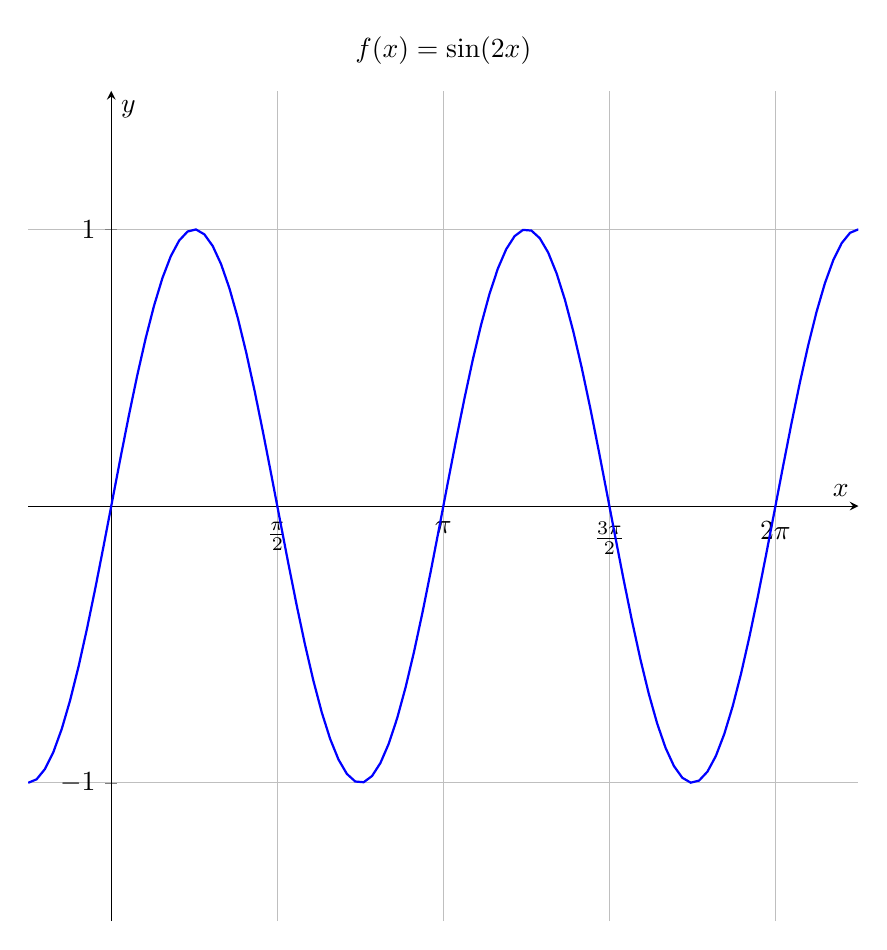
\begin{tikzpicture}
            \begin{axis}[%
                title = {$f(x) = \sin(2x)$},
                xlabel = {$x$}, ylabel = {$y$},
                xmin = -1 * 0.25 * pi, xmax = (9 * pi) / 4,
                ymin = -1.5, ymax = 1.5,
                xtick = {
                    0, 
                    pi / 2, 
                    pi, 
                    (3 * pi) / 2,
                    2 * pi%
                    },
                xticklabels = {
                    $0$,
                    $\frac{\pi}{2}$,
                    $\pi$,
                    $\frac{3\pi}{2}$,
                    $2\pi$%
                },
                ytick = {
                    -1,
                    1
                },
                axis lines = center, grid = both,
                width = \linewidth, height = \linewidth,
                trig format plots=rad
            ]
            \addplot[color = blue, thick, domain = -1 * 0.25 * pi:9/4*pi, samples = 100]{sin(2 * x)};
            \end{axis}
        \end{tikzpicture}
    \end{minipage}
    \hspace{0.05\linewidth}
    \begin{minipage}[c]{0.45\linewidth}
                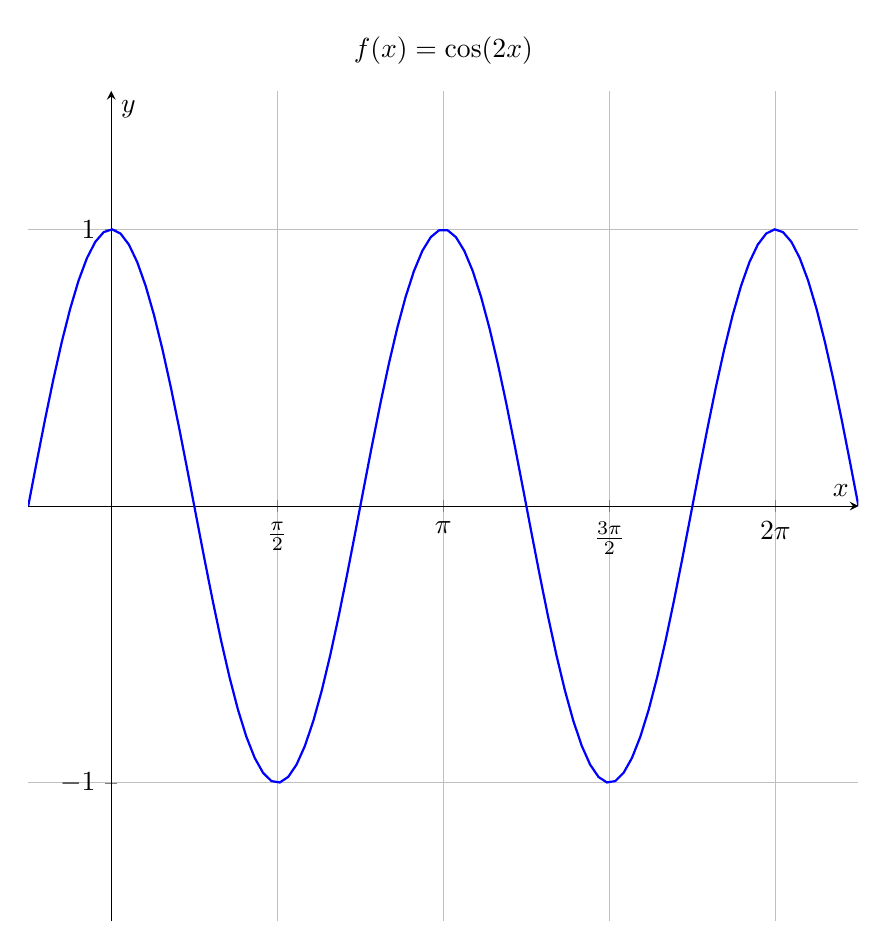
\begin{tikzpicture}
            \begin{axis}[%
                title = {$f(x) = \cos(2x)$},
                xlabel = {$x$}, ylabel = {$y$},
                xmin = -1 * 0.25 * pi, xmax = (9 * pi) / 4,
                ymin = -1.5, ymax = 1.5,
                xtick = {
                    0, 
                    pi / 2, 
                    pi, 
                    (3 * pi) / 2,
                    2 * pi%
                    },
                xticklabels = {
                    $0$,
                    $\frac{\pi}{2}$,
                    $\pi$,
                    $\frac{3\pi}{2}$,
                    $2\pi$%
                },
                ytick = {
                    -1,
                    1
                },
                axis lines = center, grid = both,
                width = \linewidth, height = \linewidth,
                trig format plots=rad
            ]
            \addplot[color = blue, thick, domain = -1 * 0.25 * pi:9/4*pi, samples = 100]{cos(2 * x)};
            \end{axis}
        \end{tikzpicture}
    \end{minipage}
\end{center}
The sine function, once again, begins at $(0,0)$ and points up. However, notice what's happeneing. There seems to be an extra wave. 

The function still points up and has a height of $y = 0$ at $x = 2\pi$, but it's \textbf{not the first occurance of it}. The first time it happens is actually at $x = \pi$.

For that reason, the frequency of $\sin(2x)$ is $\pi$ instead of $2\pi$.

The same applies for the cosine function. It begins at $(0,1)$ and points down. It has a height of $y = 1$ and also points down at at $x = 2\pi$, but it's \textbf{not the first occurance}.

Like the sine function, it reaches its first reset at $x = \pi$. Therefore, it also has a period of $\pi$.

Give this next one a shot. Before I reveal the answer on the next page, try determining the period yourself.
\begin{center}
    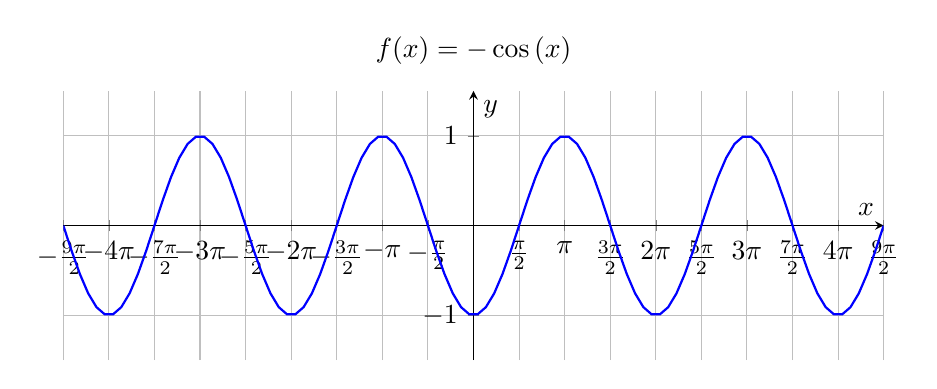
\begin{tikzpicture}
        \begin{axis}[%
            title = {$f(x) = -\cos\left(x\right)$},
            xlabel = {$x$}, ylabel = {$y$},
            xmin = -1 * (9 / 2) * pi, xmax = (9 / 2) * pi,
            ymin = -1.5, ymax = 1.5,
            xtick = {
                -1 * (9 * pi) / 2,
                -1 * 4 * pi,
                -1 * (7 * pi) / 2,
                -1 * 3 * pi,
                -1 * (5 * pi) / 2,
                -1 * 2 * pi,
                -1 * (3 * pi) / 2,
                -1 * pi,
                -1 * pi / 2,
                0, 
                pi / 2, 
                pi, 
                (3 * pi) / 2,
                2 * pi,
                (5 * pi) / 2,
                3 * pi,
                (7 * pi) / 2,
                4 * pi,
                (9 * pi) / 2%
                },
            xticklabels = {
                $-\frac{9\pi}{2}$,
                $-4\pi$,
                $-\frac{7\pi}{2}$,
                $-3\pi$,
                $-\frac{5\pi}{2}$,
                $-2\pi$,
                $-\frac{3\pi}{2}$,
                $-\pi$,
                $-\frac{\pi}{2}$,
                $0$,
                $\frac{\pi}{2}$,
                $\pi$,
                $\frac{3\pi}{2}$,
                $2\pi$,
                $\frac{5\pi}{2}$,
                $3\pi$,
                $\frac{7\pi}{2}$,
                $4\pi$,
                $\frac{9\pi}{2}$%
            },
            ytick = {
                -1,
                1
            },
            axis lines = center, grid = both,
            width = 12cm, height = 5cm,
            trig format plots=rad
        ]
        \addplot[color = blue, thick, domain = {-1 * (9 * pi) / 2}:{(9 / 2) * pi}, samples = 100]{-1 * cos(x)};
        \end{axis}
    \end{tikzpicture}
\end{center}
This one's a bit more challenging, but the answer here is $2\pi$.

Looking at the graph, we see that it begins at $(0, -1)$ and is moving up when $x = 0$. That means we need to look for the first instance where the function returns to a height of $y = -1$ and points up. That first instance happens at $x = 2\pi$. See below for the comparrison between $x = 0$ and $x = 2\pi$.
\begin{center}
    \begin{minipage}[c]{0.45\linewidth}
        \begin{tikzpicture}
            \begin{axis}[%
                title = {$f(x) = -\cos(x)$ when $x = 0$},
                xlabel = {$x$}, ylabel = {$y$},
                xmin = -1 * 0.5 * pi, xmax = 0.5 * pi,
                ymin = -1.5, ymax = 1.5,
                xtick = {
                    -1 * 0.5 * pi,
                    -1 * 0.25 * pi,
                    0,
                    0.25 * pi,
                    0.5 * pi
                    },
                xticklabels = {
                    $-\frac{\pi}{2}$,
                    $-\frac{\pi}{4}$,
                    $0$,
                    $\frac{\pi}{4}$,
                    $\frac{\pi}{2}$%
                },
                ytick = {
                    -1,
                    1
                },
                axis lines = center, grid = both,
                width = \linewidth, height = \linewidth,
                trig format plots=rad
            ]
            \addplot[color = blue, thick, domain = -1 * 0.5 * pi:0.5 * pi, samples = 100]{-1 * cos(x)};
            \end{axis}
        \end{tikzpicture}
    \end{minipage}
    \hspace{0.05\linewidth}
    \begin{minipage}[c]{0.45\linewidth}
        \begin{tikzpicture}
            \begin{axis}[%
                title = {$f(x) = -\cos(x)$ when $x = 2\pi$},
                xlabel = {$x$}, ylabel = {$y$},
                xmin = (2.99 / 2) * pi, xmax = (5 * pi) / 2,
                ymin = -1.5, ymax = 1.5,
                xtick = {
                    (3 * pi) / 2,
                    (7 * pi) / 4,
                    2 * pi,
                    (9 * pi) / 4,
                    (5 * pi) / 2%
                    },
                xticklabels = {
                    $\frac{3\pi}{2}$,
                    $\frac{7\pi}{4}$,
                    $2\pi$,
                    $\frac{9\pi}{4}$,
                    $\frac{5\pi}{2}$%
                },
                ytick = {
                    -1,
                    1
                },
                axis lines = center, grid = both,
                width = \linewidth, height = \linewidth,
                trig format plots=rad
            ]
            \addplot[color = blue, thick, domain = {-1 * 0.5 * pi + (2 * pi)}:{0.5 * pi + (2 * pi)}, samples = 100]{-1 * cos(x)};
            \end{axis}
        \end{tikzpicture}
    \end{minipage}
\end{center}
They look identical. You may have noticed that the function also looks like this at $x = 4\pi$, $x = 6\pi$, and $x = 8\pi$. But those points are irrelevant when trying to find the period. We only want the \textbf{first} occurance, and that happens at $x = 2\pi$.

I tried to trick you by extending the graph into the negative $x$-direction, introducing multiple potential choices for the period and flipping the cosine function upside down. Congratulations if you saw through it. Don't worry if you didn't. This was \textit{supposed to be} a curveball.

Before I continue to finding the period of the tangent function, I have one more problem I'd like to show you. Take a look at this one and see if you can work out what the period is.
\begin{center}
    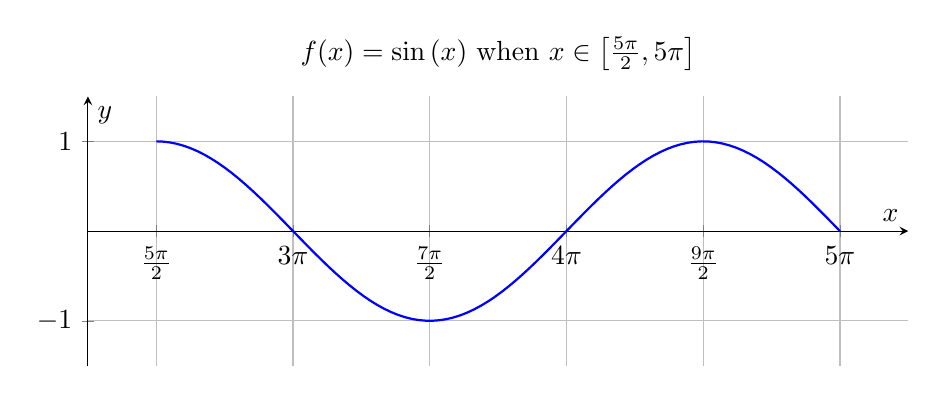
\begin{tikzpicture}
        \begin{axis}[%
            title = {$f(x) = \sin\left(x\right)$ when $x \in \left[\frac{5\pi}{2}, 5\pi \right]$},
            xlabel = {$x$}, ylabel = {$y$},
            xmin = (4.5 / 2) * pi, xmax = {5.25 * pi},
            ymin = -1.5, ymax = 1.5,
            xtick = {
                (5 * pi) / 2,
                3 * pi,
                (7 * pi) / 2,
                4 * pi,
                (9 * pi) / 2,
                5 * pi%
                },
            xticklabels = {
                $\frac{5\pi}{2}$,
                $3\pi$,
                $\frac{7\pi}{2}$,
                $4\pi$,
                $\frac{9\pi}{2}$,
                $5\pi$%
            },
            ytick = {
                -1,
                1
            },
            axis lines = center, grid = both,
            width = 12cm, height = 5cm,
            trig format plots=rad
        ]
        \addplot[color = blue, thick, domain = {(5 * pi) / 2}:{5 * pi}, samples = 100]{sin(x)};
        \end{axis}
    \end{tikzpicture}
\end{center}
This problem is challenging because I didn't give the value of $f(x)$ for $x = 0$ \textit{or} $x = 2\pi$. However, the method you use for finding the period is the exact same. In this example, I'll use the value of $f(x)$ when $x = 3\pi$.

When $x = 3\pi$, the function has a $y$ value of $y = 0$ and is pointing down. That means I need to find the first occurance of the function that returns to a height of $y = 0$ and also points down. That happens at $x = 5\pi$.

Now, to find the period, I just need to subtract the first occurance by the initial observation. That means $5\pi - 3\pi$. Subtracting gives a period of $2\pi$.

As you get better at determining the period of a trigonometric function, you won't even need much to identify. With the previous example, for instance, we could find the period in a different way.

Step 1: Observe that the function has a height of $y = 1$ and points down when $x = \frac{5\pi}{2}$.

Step 2: Observe that the function reaches a height of $y = 0$ at $x = 3\pi$.

Step 3: Remember that a sine function ossilates smoothly and evenly between $y = -1$ and $y = 1$. That means, if we started at $y = 1$ and ended at $y = 0$ after moving horizontally by $\frac{\pi}{2}$, we can predict what the graph will look like.
\begin{center}
    \begin{minipage}[c]{0.3\linewidth}
        \begin{tabular}{ c | c }
            $x$ & $f(x) = \sin(x)$ \\
            \hline
            $\frac{5\pi}{2}$ & $1$ \\
            \hline
            $3\pi$ & $0$ \\
            \hline
            $\frac{7\pi}{2}$ & $-1$ \\
            \hline
            $4\pi$ & $0$ \\
            \hline
            $\frac{9\pi}{2}$ & $1$ \\
        \end{tabular}
    \end{minipage}
    \begin{minipage}[c]{0.69\linewidth}
        Step 4: With this table, observe that the height of the function at $x = \frac{9\pi}{2}$ is $y = 1$, which is the same height at $x = \frac{5\pi}{2}$. 
        \\ \\
        Step 5: Take $\frac{9\pi}{2} - \frac{5\pi}{2}$ to find the period. When we subtract, we get $\frac{4\pi}{2}$, which is $2\pi$. 
    \end{minipage}
\end{center}
We got the same result as before, but with only $\frac{\pi}{2}$ of the graph to work with.